\documentclass{article}
\usepackage{iclr2027_conference,times}

\usepackage{amsmath,amssymb,amsthm}
\usepackage{booktabs}
\usepackage{graphicx}
\usepackage{microtype}
\usepackage{url}

\newtheorem{lemma}{Lemma}
\newtheorem{proposition}{Proposition}
\theoremstyle{definition}
\newtheorem{definition}{Definition}

\newcommand{\bwe}{\ensuremath{\eta}}

\title{Which Interpretability Diagnostics Track Program\\
Correctness? Evidence from a Compiled Transformer\\
with Floating-Point Ground Truth}

\author{Anonymous authors\\Paper under double-blind review}

\begin{document}
\maketitle

\begin{abstract}
Mechanistic interpretability certifies that a network ``implements an algorithm''
using diagnostics computed from its behavioural surface: attention that is
one-hot or low-entropy, outputs that are finite, predictions invariant to
pruning, heads whose ablation is critical. Whether these track program-level
correctness is an empirical question that needs ground truth of a kind trained
models cannot supply. We build it. We compile the triangular solves of LU-based
matrix inversion into transformer weights at binary64 precision, so that both
the intended program structure \emph{and} its floating-point semantics are known
before execution, and we derive a \emph{certified-exact} oracle for the position
every attention lookup should fetch. Across 30 compiled programs and 360
execution configurations we find that diagnosticity varies by an order of
magnitude and does not match how these signals are used in practice: output
finiteness is close to useless (AUC $0.571$), exact one-hotness and low entropy
are moderate ($0.826$, $0.755$), and invariance of the downstream prediction is
the strongest ($0.964$). Head-ablation criticality is a poor estimator of the
compiler's own functional labels (precision $0.556$, recall $0.349$ against a
$49\%$ base rate). We further prove a margin bound showing that exact
hard-attention positional addressing needs about $2\log_2 P + 4.4$ significand
bits to address $P$ positions, that the attention temperature cancels from this
condition, and---contrary to a natural conjecture---that bounded-magnitude
re-encoding does not relax it. Our testbed is not a solver; it is an instrument,
and it says which reassurance signals deserve trust.
\end{abstract}

% =============================================================================
\section{Introduction}
% =============================================================================

A recurring claim in mechanistic interpretability is that some network
``implements'' a particular algorithm. The evidence offered is usually indirect:
attention distributions that are effectively one-hot, low attention entropy,
outputs that remain finite and plausible, predictions that survive pruning or
quantization, and ablation studies showing that particular heads are critical
\citep{clark2019bert,voita2019analyzing,elhage2021framework,wang2023ioi}. These
are \emph{proxies}. They are cheap, they are widely used, and how well they track
correctness is not known, because establishing it requires a system whose
intended computation is known independently of the network's behaviour.

Compiled transformers supply part of that ground truth. Tracr
\citep{lindner2023tracr} compiles RASP programs \citep{weiss2021thinking} into
weights; ALTA \citep{shaw2025alta} and looped constructions
\citep{giannou2023looped} extend the compilation target; InterpBench
\citep{gupta2024interpbench} and MIB \citep{mueller2025mib} use known-circuit
models to score interpretability methods. What none of them provides is a
\emph{numerical} axis. Their programs are symbolic, so there is no notion of the
computation being carried out to a stated accuracy, and no way to perturb
precision and ask whether the program is still computing the right values.

We add that axis. CRAFT compiles the forward and backward substitution of
LU-based matrix inversion into transformer weights at binary64, for symmetric
positive-definite Laplacian systems. Because the program is emitted rather than
learned, three things are known before any execution: which dimension holds which
intermediate quantity, which attention head is supposed to fetch from which
position, and what the exact arithmetic result should be. Perturbing the
execution---dtype, quantization, pruning, head ablation---then moves the program
away from correctness in a measurable way, while the behavioural proxies can be
read off exactly as a practitioner would read them.

This yields a question that can actually be answered:

\begin{quote}
When a numerical program is compiled into transformer weights with ground-truth
operation labels available, which of the standard diagnostics used to certify
that a transformer ``implements an algorithm'' actually track program-level
correctness under precision and quantization perturbation, and which give false
reassurance?
\end{quote}

Our contributions:

\begin{enumerate}
\item \textbf{A ground-truth testbed with a certified-exact oracle}
(\S\ref{sec:testbed}). We derive, for every attention lookup, the position the
program must fetch, certified by a rounding-error bound with exact rational
fallback. Over $104{,}381$ lookup decisions, $98.1\%$ are certified directly and
the rest are resolved exactly. The oracle is a property of the compiled program,
not of any particular run, which is what lets us score a perturbed execution
without circularity.

\item \textbf{A measurement of proxy diagnosticity} (\S\ref{sec:main}). Across 30
programs $\times$ 12 configurations we report, for each proxy, its green rate on
correct runs, its false-reassurance rate, a likelihood ratio, and the AUC of its
continuous value against compiler-labelled correctness. The spread is large and
the ranking is not the one practice assumes.

\item \textbf{A head-ablation audit against compiler labels}
(\S\ref{sec:ablation}). Ablation criticality recovers the compiler's own
lookup/passthrough labels with precision $0.556$ and recall $0.349$.

\item \textbf{A precision requirement for compiled attention addressing}
(\S\ref{sec:precision}). Exact selection up to position $P$ needs roughly
$2\log_2 P + 4.4$ significand bits. The attention temperature $K$ cancels
entirely from the precision condition and enters only a dynamic-range condition,
so the large $K$ used in constructive results buys nothing and costs range. We
also show that normalizing the positional encoding does \emph{not} help, because
it shrinks the margin exactly as fast as the magnitudes.

\item \textbf{Evidence that the compiled program executes run-time inputs}
(\S\ref{sec:runtime}), so the proxy results are about a solver and not about a
replayed constant.
\end{enumerate}

We are explicit that CRAFT is not a useful solver---it is about five orders of
magnitude slower than a library call---and that its compiler accepts only
coefficients known at build time. It is an instrument. Its value is that every
number it produces can be checked.

% =============================================================================
\section{Related work}
% =============================================================================

\paragraph{Compiled and constructive transformers.} RASP
\citep{weiss2021thinking} and Tracr \citep{lindner2023tracr} compile symbolic
programs into transformer weights; ALTA \citep{shaw2025alta} targets a lower-level
assembly; \citet{giannou2023looped} build programmable looped transformers.
Expressivity results establish what hard-attention transformers can represent
\citep{perez2019turing,perez2021attention,hahn2020theoretical,barcelo2024logical,merrill2023parallelism,merrill2023logic},
surveyed by \citet{strobl2024formal}. These are stated over the reals or with
idealized precision; our contribution is to ask what precision the constructions
actually require.

\paragraph{Interpretability evaluation with known ground truth.} InterpBench
\citep{gupta2024interpbench} and MIB \citep{mueller2025mib} evaluate circuit
discovery against known structure; ACDC \citep{conmy2023acdc} and causal
scrubbing \citep{chan2022causalscrubbing} are the methods being evaluated.
\citet{miller2024faithfulness} show circuit-faithfulness metrics are sensitive to
methodological choices. Our axis is complementary and, to our knowledge, absent:
these benchmarks have no notion of a program being numerically wrong.

\paragraph{Architecture.} A controller that mutates an external memory between
steps is a Neural Turing Machine / DNC
\citep{graves2014neural,graves2016hybrid}; our runner-plus-cache is that design.
Our attention lookup is 2-D maximum inner product search, i.e.\ the dynamic
convex hull trick \citep{overmars1981maintenance,brodal2002dynamic,li2026lichao};
attention-as-MIPS is also the basis of LSH attention
\citep{shrivastava2014asymmetric,kitaev2020reformer}.

\paragraph{Numerical analysis.} The backward error we measure is the classical
normwise quantity of \citet{rigal1967compatibility}, with
\citet{oettli1964compatibility} as the componentwise ancestor; see
\citet[Thm~7.1]{higham2002accuracy}. LU stability and growth factors are
classical \citep{wilkinson1961error,wilkinson1963rounding,higham2002accuracy}.
Our $\bwe$ measurements confirm this theory rather than extending it; we report
them as calibration. Verified numerics
\citep{rump1983solving,rump1999intlab,rump2010verification,ogita2005accurate}
and machine-checked floating-point proofs
\citep{boldo2011flocq,daumas2010certification,roux2016formal,kellison2023laproof,kwan2024formalizing}
give stronger guarantees for linear solvers than an a-posteriori certificate;
our claim is not to compete with them but to apply their standard of evidence
inside a transformer.

\paragraph{Quantization and pruning.} We use per-tensor and per-channel int8
\citep{jacob2018quantization,krishnamoorthi2018quantizing,nagel2021whitepaper,dettmers2022llmint8},
bfloat16 \citep{kalamkar2019bfloat16,burgess2019bfloat16}, and magnitude pruning
\citep{han2015learning,han2016deepcompression,frankle2019lottery}.

% =============================================================================
\section{The testbed and its oracle}\label{sec:testbed}
% =============================================================================

\paragraph{What is compiled.} The host computes the Doolittle factors
$\hat L,\hat U$ of $A_{FF}$ once at build time and bakes them into token
embeddings. The transformer executes forward and backward substitution token by
token. A runner threads values between steps through the KV cache, supplying
$b_i$ at the \texttt{rhs}$_i$ token and $y_i$ at \texttt{bck}$_i$. We do not
claim the factorization is executed by the network.

\paragraph{Scope.} The compiler accepts only coefficients known at build time.
No compiled program here can express pivoting, input-dependent control flow, or
input-dependent coefficients, and each matrix is compiled separately. This is a
ceiling on the framework, and it bounds what ``a transformer executes a numerical
routine'' can mean in this setting.

\paragraph{Two populations.} Of 154 circuits in our suite, the target node is a
\emph{fixed} source node in 12. For those the compiler emits a direct source
read: the substitution machinery is compiled and scheduled but never exercised,
and 88 free-variable solve steps are built and never run. Those 12 attain zero
downstream error without executing a solve. We report every execution result on
the 142 that do execute, and we flag this because it is exactly the failure mode
a testbed should catch: a program can pass an application-level metric without
running.

\paragraph{The oracle.} Let $s(p)=\langle k_p, q_t\rangle$ be the attention score
at position $p$. The position the program \emph{must} fetch is
$\arg\max_p s(p)$ evaluated exactly. Computing that in rational arithmetic at
every lookup is expensive, so we certify instead: if the float64 winning margin
exceeds a bound on the accumulated rounding error of a two-term dot product, the
computed $\arg\max$ is provably the exact one; otherwise we recompute that row
with \texttt{Fraction}. Over $104{,}381$ lookup decisions on compiler-labelled
lookup heads, $98.1\%$ were certified directly (minimum $95.7\%$ per program) and
$927$ required the exact fallback.

This matters for validity. Defining correctness as ``selects what the float64 run
selected'' would be circular for the precision arm, since any dtype change would
then be incorrect by construction. Our oracle is a property of the compiled
program, so a perturbed configuration is scored against what the program
\emph{means}.

\paragraph{Head labels.} The compiler assigns each attention head a role:
\emph{lookup} heads implement a scheduled fetch, \emph{passthrough} heads carry
slot contents forward using an erase query. We read these labels from the
compiler's allocation record. This distinction is load-bearing: pooling the two
makes exact one-hotness unattainable even on provably correct runs (it caps at
$0.22$), which would make the proxy unmeasurable. All proxies below are computed
on lookup heads.

% =============================================================================
\section{The compiled program executes run-time inputs}\label{sec:runtime}
% =============================================================================

If the compiled model only ever ran on one input, its attention pattern would say
nothing about computation. We therefore drive each program with six families of
right-hand side, \textbf{with no recompilation between them}: columns of the
identity, the physical source-driven $b$, i.i.d.\ Gaussian, wide-dynamic-range
vectors spanning $10^{-8}$ to $10^{8}$, the all-ones forcing vector solved
in-model, and a vector aligned with the smallest singular direction of $A$.

Over 40 matrices and $1{,}163$ solves, the maximum per-column normwise backward
error is $1.88\times10^{-16}\approx1.7u$ and the selector hit rate against the
oracle is exactly $1.000$ in every family; median $\bwe$ ranges from
$1.19\times10^{-17}$ to $4.16\times10^{-17}$ with no family separating from the
others (Appendix~\ref{app:runtime}). The program computes a genuine function of
its input, at the accuracy classical theory predicts for a triangular solve with
a growth factor near 1 \citep{higham2002accuracy}.

% =============================================================================
\section{Main result: diagnosticity varies by an order of magnitude}\label{sec:main}
% =============================================================================

\paragraph{Design.} 30 compiled programs ($n\in[3,44]$ unknowns) $\times$ 12
execution configurations: dtype $\{$f64, f32, bf16, f16$\}$; quantization
$\{$per-tensor int8, per-channel int8$\}$; and magnitude pruning at
$\{10,50,90\}\%$ computed both over all coefficients and over \emph{nonzero}
coefficients only. 360 independent cells. A run is \emph{broken} when any lookup
fetches a position other than the oracle's, or when the output is not finite.

\paragraph{Proxies.} (i) all outputs finite; (ii) softmax exactly one-hot;
(iii) attention entropy $\approx0$, computed as true Shannon entropy with no
regulariser; (iv) downstream prediction unchanged from the f64 run.

\begin{table}[t]
\caption{Proxy diagnosticity against the certified-exact compiler oracle. 30
programs, 360 configurations, 210 broken. $\mathrm{LR}_{\text{green}}
= P(\text{green}\mid\text{correct})/P(\text{green}\mid\text{broken})$; $1.0$ is
uninformative. AUC is rank discriminability of the proxy's continuous value;
$0.5$ is chance. Intervals are cluster bootstraps over programs.}
\label{tab:proxies}
\begin{center}
\begin{tabular}{lcccc}
\toprule
Proxy & $P(\text{green}\mid\text{correct})$ & $P(\text{green}\mid\text{broken})$
& $\mathrm{LR}_{\text{green}}$ & AUC \\
\midrule
outputs all finite       & $1.000$ & $0.857$ & $1.17$  & $0.571$ \\
attention entropy $\approx 0$ & $1.000$ & $0.490$ & $2.04$  & $0.755$ \\
softmax exactly one-hot  & $1.000$ & $0.348$ & $2.88$  & $0.826$ \\
prediction unchanged     & $1.000$ & $0.071$ & $14.00$ & $\mathbf{0.964}$ \\
\midrule
all four simultaneously  & --- & $0.019$ & --- & --- \\
\bottomrule
\end{tabular}
\end{center}
\end{table}

Table~\ref{tab:proxies} is the paper's main result, and it is more discriminating
than a blanket ``proxies fail''. Every proxy is green on every correct run, so
none produces false alarms. They differ sharply in what a green reading is worth:

\begin{itemize}
\item \textbf{Output finiteness is close to useless} (AUC $0.571$, LR $1.17$). It
stays green in $85.7\%$ of runs in which the program provably fetches wrong
values. It is also the cheapest and most commonly applied sanity check.

\item \textbf{Exact one-hotness and near-zero entropy are moderate}
($0.826$, $0.755$). Notably, these are only measurable at all once heads are
separated by compiler role; pooled over all heads they are degenerate.

\item \textbf{Prediction invariance is the strongest signal} (AUC $0.964$,
LR $14.0$), despite being measured on a coarse 101-point output grid. This is the
opposite of what a mechanistic account would suggest---an end-to-end behavioural
check outperforms three internal, mechanism-flavoured ones.
\end{itemize}

Only $1.9\%$ of broken runs are green on all four simultaneously, so a
\emph{conjunction} of diagnostics is far safer than any single one. That is an
actionable recommendation, and it is not what single-proxy practice does.

\begin{figure}[t]
\begin{center}
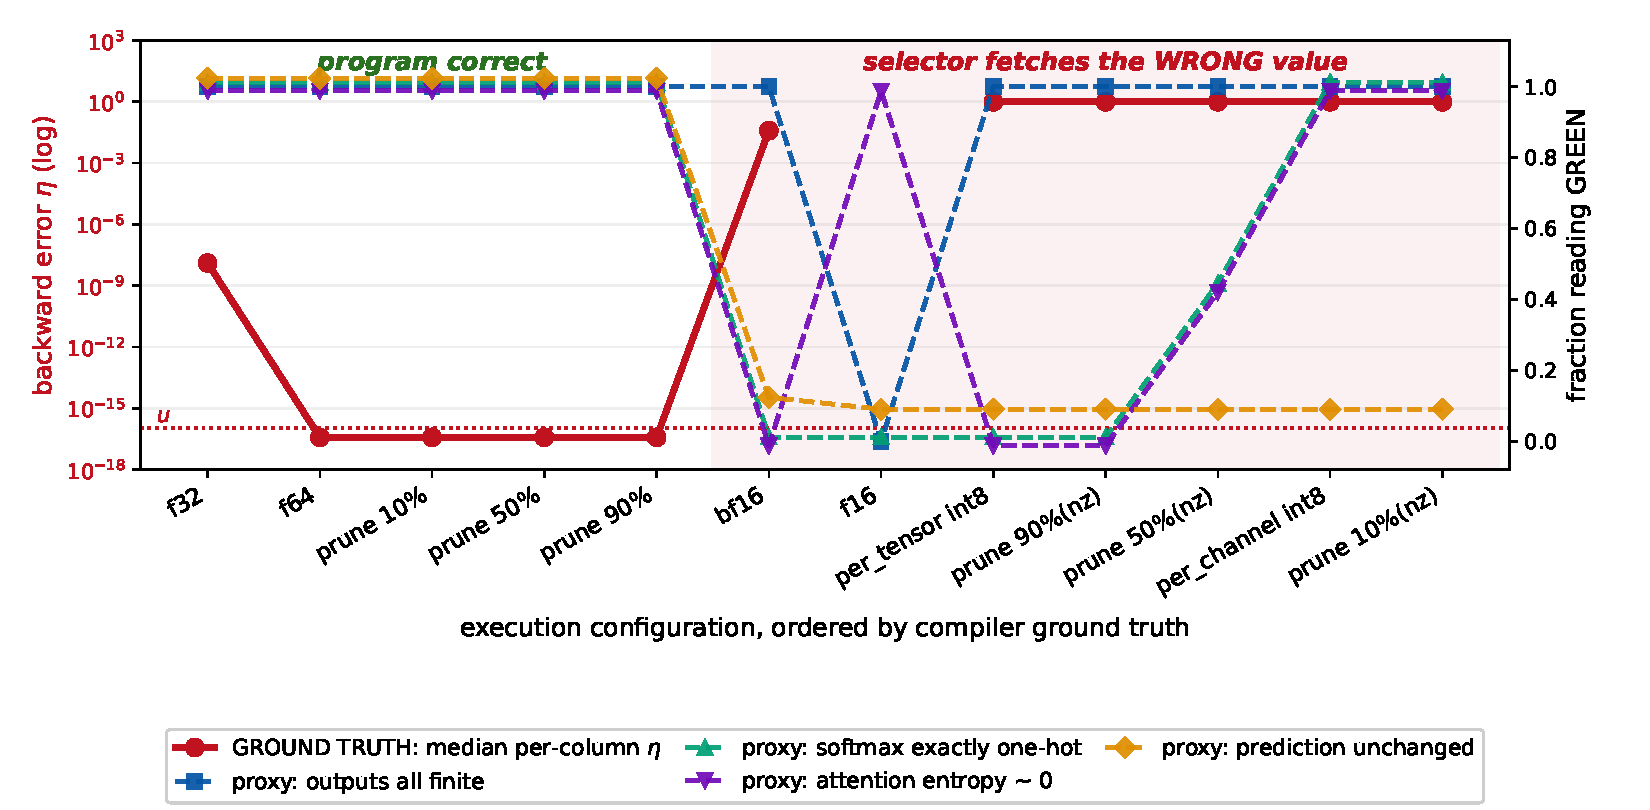
\includegraphics[width=\textwidth]{fig1_proxy_dissociation.pdf}
\end{center}
\caption{Ground truth (red, left log axis) versus the four proxies (right axis)
across execution configurations ordered by compiler-labelled correctness. In the
shaded region the selector provably fetches wrong values while proxy curves
remain high---most conspicuously output finiteness.}
\label{fig:main}
\end{figure}

\paragraph{Pruning invariance is structural sparsity.} Pruning $10/50/90\%$ of
\emph{all} coefficients leaves execution bit-identical ($\bwe=3.9\times10^{-17}$,
hit rate $1.000$). Pruning $10\%$ of the \emph{nonzero} coefficients destroys it
($\bwe=1.0$, hit rate $0.130$). Reports of extreme pruning invariance in compiled
models can therefore be measuring how sparse the emitted tensor already is. The
distinction costs one line of code and reverses the conclusion.

\paragraph{The attention temperature is not the mechanism.} A natural explanation
for quantization collapse is that a large attention scale $K$ dominates the
tensor range and rounds the arithmetic coefficients away. We tested it by
recompiling at $K\in\{10^{10},10^{8},10^{6},10^{4}\}$: the int8 hit rate moves
from $0.898$ to $0.903$ and $\bwe$ stays at $1.00$ throughout. Six orders of
magnitude of $K$ change nothing, consistent with \S\ref{sec:precision} where $K$
cancels analytically. Per-channel int8 \citep{dettmers2022llmint8} does not
rescue execution either.

% =============================================================================
\section{Head-ablation criticality against compiler labels}\label{sec:ablation}
% =============================================================================

Ablation is the standard tool for attributing function to heads. With compiler
labels we can score it directly. We zero each head's output contribution in turn
across 8 programs (174 labelled heads) and ask whether the prediction changes.

\begin{table}[t]
\caption{Head ablation versus the compiler's own functional labels.}
\label{tab:ablation}
\begin{center}
\begin{tabular}{lccc}
\toprule
Compiler label & heads & ablation changes prediction & ablation breaks program \\
\midrule
lookup      & $86$ & $30\ (34.9\%)$ & $47\ (54.7\%)$ \\
passthrough & $88$ & $24\ (27.3\%)$ & $61\ (69.3\%)$ \\
\bottomrule
\end{tabular}
\end{center}
\end{table}

Treating ``ablation changes the prediction'' as a detector for ``the compiler
assigned this head a lookup role'' gives precision $0.556$ and recall $0.349$,
against a base rate of $86/174=49.4\%$ lookup heads. Ablation criticality is
close to uninformative about compiler-assigned role here: it misses two thirds of
the heads that genuinely perform scheduled fetches, and nearly half of the heads
it flags are passthrough. Two mechanisms explain this without any appeal to
redundancy: many lookup heads feed quantities the coarse output grid cannot
resolve, and passthrough heads are load-bearing for state propagation even though
they compute nothing.

% =============================================================================
\section{How much precision does compiled addressing need?}\label{sec:precision}
% =============================================================================

Constructive transformer results are stated over the reals. The following says
what they cost in bits. The compiler scales the query by $K$, so with keys
$k_p=(2p,\,-p^2+\alpha g(p))$ and query $q_t=K'(t,1)$, $K'=K\sqrt{d_h}$,
\[
s(p) = K'\bigl(2pt-p^2+\alpha g(p)\bigr)
     = K'\bigl(t^2-(t-p)^2+\alpha g(p)\bigr),
\]
and the $t^2$ term cancels from every pairwise comparison.

\begin{lemma}[Selector exactness]\label{lem:margin}
Let $0\le g<1/\ln2$ and $0<\alpha<\ln 2$, and write $M=1-\alpha/\ln2$. For
$p\neq t$, $s(t)-s(p)\ge K'M$. If all positions satisfy $p,t\le P$ with $P\ge1$,
then the computed $\arg\max$ in a binary floating-point format with unit roundoff
$u$ and largest finite value $\Omega$ equals the exact $\arg\max$ whenever
\[
\text{(precision)}\quad P<\sqrt{\frac{M}{12u}},
\qquad\text{and}\qquad
\text{(range)}\quad P<\sqrt{\frac{\Omega}{3K'}} .
\]
The scale $K'$ cancels from the precision condition and appears only in the range
condition.
\end{lemma}

A proof is in Appendix~\ref{app:proof}. Equivalently, addressing $P$ positions
exactly requires about $2\log_2 P+\log_2(12/M)\approx 2\log_2 P+4.4$ significand
bits: $11.0$ bits for $P=10$, $22.9$ for $P=601$, $31.0$ for $P=10^4$.

\begin{table}[t]
\caption{Predicted ceilings at the production scale $K=10^{10}$ against measured
first-failure positions. The bound is sufficient, hence conservative where
precision binds; for float16 the \emph{range} condition binds and predicts
immediate failure, which is what occurs.}
\label{tab:precision}
\begin{center}
\begin{tabular}{lccccc}
\toprule
Format & $P_{\text{precision}}$ & $P_{\text{range}}$ & binding & predicted $P$ & measured first failure \\
\midrule
float64  & $2.06\times10^{7}$ & $7.7\times10^{148}$ & precision & $2.06\times10^{7}$ & none up to $4\times10^{6}$ \\
float32  & $891$              & $1.1\times10^{14}$  & precision & $891$              & $3898$ \\
bfloat16 & $4.92$             & $1.1\times10^{14}$  & precision & $4.92$             & $15$ \\
float16  & $9.84$             & $\mathbf{0.0015}$   & \textbf{range} & $\mathbf{0.0015}$ & $\mathbf{1}$ \\
\bottomrule
\end{tabular}
\end{center}
\end{table}

\paragraph{Bounded-magnitude re-encoding does not help.} It is tempting to blame
low-precision failure on unbounded score magnitude and propose normalizing
positions, $p\mapsto p/P$. This does not work, and the reason generalizes:
normalization divides the margin by $P^2$ exactly as it divides the magnitudes,
leaving the relative gap unchanged, so the condition becomes $P<1/\sqrt{2u}$ ---
the same $O(u^{-1/2})$ scaling. Empirically, the normalized encoding first fails
at position $15$ in bfloat16, identical to the production encoding. The
requirement is intrinsic to quadratic positional keys, not an artifact of a badly
chosen constant.

\paragraph{Consequence.} The large attention temperature used to force
hard attention is a pure liability: it cannot buy exactness (Lemma~\ref{lem:margin})
and it shrinks the representable position range. Compiled-transformer
constructions that assume real arithmetic should state a precision budget, and
this lemma gives it.

\begin{table}[t]
\caption{Ground truth by execution configuration (30 programs each). A
configuration is broken when any lookup deviates from the oracle. Note the
separation between pruning computed over all coefficients and over nonzero
coefficients only, and that per-channel int8 is \emph{worse} here than
per-tensor.}
\label{tab:byconfig}
\begin{center}
\begin{tabular}{lccc|lccc}
\toprule
Config & frac.\ broken & med.\ hit & med.\ $\bwe$ &
Config & frac.\ broken & med.\ hit & med.\ $\bwe$ \\
\midrule
f64        & $0.00$ & $1.000$ & $3.9\!\times\!10^{-17}$ & bf16             & $1.00$ & $0.915$ & $3.9\!\times\!10^{-2}$ \\
f32        & $0.00$ & $1.000$ & $1.3\!\times\!10^{-8}$  & f16              & $1.00$ & $0.628$ & $\infty$ \\
prune 10\% & $0.00$ & $1.000$ & $3.9\!\times\!10^{-17}$ & per-tensor int8  & $1.00$ & $0.628$ & $1.00$ \\
prune 50\% & $0.00$ & $1.000$ & $3.9\!\times\!10^{-17}$ & per-channel int8 & $1.00$ & $0.241$ & $1.00$ \\
prune 90\% & $0.00$ & $1.000$ & $3.9\!\times\!10^{-17}$ & prune 10\%(nz)   & $1.00$ & $0.130$ & $1.00$ \\
\bottomrule
\end{tabular}
\end{center}
\end{table}

Table~\ref{tab:byconfig} gives the ground truth per configuration. Two features
are worth noting. First, the correct/broken boundary is sharp: every
configuration is either entirely correct across all 30 programs or entirely
broken, which is what one expects when correctness is governed by a margin
condition rather than by accumulated noise. Second, the \emph{severity} ordering
is not the intuitive one---per-channel int8 degrades the selector further than
per-tensor, and nonzero-pruning at $10\%$ is the most destructive configuration
tested, worse than dropping to float16.

% =============================================================================
\section{Discussion}\label{sec:discussion}
% =============================================================================

Our results suggest three concrete changes to how compiled-model evidence is
reported.

\textbf{Report a conjunction, not a single proxy.} No single diagnostic is safe:
the best one still reads green in $7\%$ of broken runs, and the most commonly
used one in $86\%$. All four together fail only $1.9\%$ of the time. Since the
proxies are cheap and largely independent, reporting them jointly is close to
free.

\textbf{Separate heads by role before measuring internal proxies.} One-hotness
and entropy are unmeasurable when lookup and passthrough heads are pooled---the
pooled statistic never reaches the value a correct run attains. Any claim of the
form ``attention is one-hot, so the model is doing lookup'' needs the head
partition to be stated. In a compiled model it is available; in a trained model
it is precisely what is being inferred, which is a reason for caution.

\textbf{State a precision budget.} Constructive transformer results assume real
arithmetic. Lemma~\ref{lem:margin} converts that assumption into a number of
significand bits, and shows that the standard trick of raising the attention
temperature does not buy accuracy---it only costs dynamic range. A construction
that addresses $10^4$ positions needs $31$ bits of significand and therefore
cannot be executed in any $16$-bit format, however it is scaled.

Finally, a methodological point. Two results here were only visible because the
ground truth was a \emph{compiler} rather than a reference run: that $12$ of
$154$ programs pass the application metric without executing, and that pruning
invariance was a statement about tensor sparsity. Both would have been reported
as successes by a pipeline that compared against its own float64 trace.

% =============================================================================
\section{Limitations}\label{sec:limitations}
% =============================================================================

\textbf{Compiled, not trained.} Our object of study is a hand-compiled, untrained,
structurally sparse network. We show which proxies track correctness \emph{in a
setting where correctness is checkable}; whether the same ranking holds for
gradient-trained models is not established here, and is the main threat to
external validity. We think the finiteness result is likeliest to transfer (it is
a property of the metric, not of the network) and the ablation result least.

\textbf{Perturbations are strong.} int8, bfloat16 and nonzero-pruning are
aggressive. We do not claim practitioners believe these proxies certify numerical
correctness under quantization; we claim that when they \emph{are} read as health
signals, their diagnosticity differs by an order of magnitude, and that ordering
was not previously measurable.

\textbf{Scale and scope.} $n\le 44$ unknowns, one compiler, one architecture
family, one program family (triangular substitution), build-time-constant
coefficients only, no pivoting. Ablation covers 174 labelled heads on 8 programs.

\textbf{Reduction order depends on a MILP solve.} Compiling one circuit under
five solver configurations yields five distinct weight files; for one of four
circuits tested the \emph{executed result} changed by $1.84$ ulp, traceable to a
different slot assignment and hence a different FFN reduction order. Bitwise
reproducibility claims about compiled models must be scoped to a fixed schedule
(Appendix~\ref{app:milp}).

\textbf{Not a solver.} About $10^5\times$ slower than a library solve.

% =============================================================================
\section*{Reproducibility statement}
% =============================================================================

All results come from scripts released with the submission, run on CPU in
float64 under a single pinned source tree. Appendix~\ref{app:proof} contains the
proof of Lemma~\ref{lem:margin}; Appendix~\ref{app:runtime} the full run-time
right-hand-side table; Appendix~\ref{app:milp} the schedule-stability data;
Appendix~\ref{app:repro} the environment, per-script runtimes and entry points.
The oracle's certification rate and exact-fallback counts are reported per
program so the ground truth itself can be audited.

\bibliography{refs_verified}
\bibliographystyle{iclr2027_conference}

\appendix
% =============================================================================
\section{Proof of Lemma~\ref{lem:margin}}\label{app:proof}
% =============================================================================

\textbf{Exact margin.} For $p\neq t$,
$s(t)-s(p)=K'\left[(t-p)^2+\alpha\bigl(g(t)-g(p)\bigr)\right]$. Since $p\neq t$
are integers, $(t-p)^2\ge1$; since $0\le g<1/\ln2$, $|g(t)-g(p)|<1/\ln2$. Hence
$s(t)-s(p)\ge K'(1-\alpha/\ln2)=K'M>0$ for $\alpha<\ln2$. Numerically, with
$\alpha=0.3$ we have $M=0.5672$, and the minimum exact gap measured over
$t\in[1,3\times10^5]$ is $0.9996$, so the bound holds with room.

\textbf{Rounding.} Each score is a two-term dot product. Under the standard model
$\mathrm{fl}(a\ \mathrm{op}\ b)=(a\ \mathrm{op}\ b)(1+\delta)$, $|\delta|\le u$,
two products and one addition give
$|\mathrm{fl}(s(p))-s(p)|\le\gamma_2 S_p$ with $\gamma_2=2u/(1-2u)$ and
$S_p=K'\bigl(|2pt|+|-p^2+\alpha g(p)|\bigr)$, the absolute-value sum that bounds
cancellation. For $p,t\le P$ and $P\ge1$, $S_p\le 3K'P^2$.

\textbf{Precision condition.} The computed $\arg\max$ is exact if the exact
margin exceeds the worst combined perturbation of the two scores compared:
$K'M>\gamma_2(S_t+S_p)$, which is implied by $M>6\gamma_2P^2$. Using
$\gamma_2\le2u/(1-2u)$ and $u\le\frac12$, a sufficient condition is
$M>12uP^2$, i.e.\ $P<\sqrt{M/(12u)}$. The factor $K'$ appears on both sides and
cancels. $\square$

\textbf{Range condition.} Representability requires
$\max_p|s(p)|\le3K'P^2\le\Omega$, giving $P<\sqrt{\Omega/(3K')}$, which does
depend on $K'$. The valid range is the minimum of the two conditions.

% =============================================================================
\section{Run-time right-hand sides}\label{app:runtime}
% =============================================================================

\begin{table}[h]
\caption{40 matrices, $1{,}163$ solves, no recompilation between right-hand
sides. $u=1.11\times10^{-16}$. Selector hit rate is against the certified-exact
oracle.}
\begin{center}
\begin{tabular}{lrrrr}
\toprule
RHS family & solves & $\max\bwe$ & median $\bwe$ & min selector hit \\
\midrule
identity columns $e_j$ & 243 & $1.58\times10^{-16}$ & $1.25\times10^{-17}$ & $1.000$ \\
source-driven $b$      & 40  & $1.88\times10^{-16}$ & $4.16\times10^{-17}$ & $1.000$ \\
i.i.d.\ Gaussian       & 400 & $1.64\times10^{-16}$ & $1.44\times10^{-17}$ & $1.000$ \\
wide dynamic range     & 400 & $1.78\times10^{-16}$ & $2.11\times10^{-17}$ & $1.000$ \\
all-ones, in-model     & 40  & $1.09\times10^{-16}$ & $1.36\times10^{-17}$ & $1.000$ \\
adversarial            & 40  & $1.18\times10^{-16}$ & $1.19\times10^{-17}$ & $1.000$ \\
\bottomrule
\end{tabular}
\end{center}
\end{table}

% =============================================================================
\section{Schedule stability}\label{app:milp}
% =============================================================================

Each circuit was compiled under five MILP configurations (three solver seeds, a
reduced time limit, and a different solver backend) and executed on identical
inputs. All five produce distinct weight files. For three of four circuits the
executed result is bit-identical; for one it differs by $1.84$ ulp, tracking a
third distinct slot map. The emitted program is not byte-stable across solver
configurations, and the executed result is not always bit-stable either.

% =============================================================================
\section{Downstream metric decomposition}\label{app:voltage}
% =============================================================================

The application-level readout quantizes to a $50$\,mV grid. Decomposing the error
over all 154 circuits: total $11.84$\,mV mean; readout quantization
$11.84$\,mV; target-model mismatch $0.025$\,mV; and the solve itself
$1.6\times10^{-10}$\,mV. Total and quantization error agree to four significant
figures, and the uniform-in-bin expectation is $12.5$\,mV. The metric measures
the readout budget, not solver accuracy; we use it in
\S\ref{sec:main} only as a behavioural proxy, which is the one role it can
support. We also report that $0$ of $1437$ solution entries are negative, so the
pipeline's non-negativity clamp is a no-op on the declared domain.

% =============================================================================
\section{Reproducibility details}\label{app:repro}
% =============================================================================

CPU only; float64 throughout (the attention scale overflows in float32, and the
workload is dispatch-bound rather than FLOP-bound, so no GPU is used or needed).
Compiled models are regenerated deterministically from the build scripts given a
fixed MILP configuration; see Appendix~\ref{app:milp} for the caveat. Each
program builds in $1$--$45$\,s and solves in under a second. Entry points, exact
package versions and per-script runtimes are in the released \texttt{README}.

% =============================================================================
\section{Use of large language models}\label{app:llm}
% =============================================================================

An LLM-based coding assistant was used substantially in this work and we disclose
that here in line with the conference policy. Its role was: implementing the
experiment scripts and the certified-exact oracle; running the experiments and
tabulating results; drafting and revising this manuscript; and conducting the
literature search, including retrieving and cross-checking bibliographic records.
Every citation in this paper was independently verified to exist against a
primary source (publisher DOI records, ACL Anthology, or proceedings pages)
before inclusion, and one candidate reference that could not be verified was
removed. The research questions, the experimental designs, the interpretation of
results and all scientific claims are the authors' responsibility, and the
authors have checked the derivations and re-run the reported experiments.

\end{document}
